\documentclass[5p,times]{elsarticle}

\usepackage{ecrc}
\usepackage{amsmath,amssymb,amsfonts}
\usepackage{graphicx}
\usepackage{booktabs}
\usepackage{hyperref}
\usepackage{url}
\usepackage{cite}

\volume{292}
\firstpage{1390}
\journalname{Procedia Computer Science}
\runauth{Moad Moussaoui et al.}
\jid{procs}
\jnltitlelogo{Procedia Computer Science}

\begin{document}

\begin{frontmatter}

\dochead{30th International Conference on Knowledge-Based and Intelligent Information \& Engineering Systems (KES 2026)}

\title{YOLOv11-Based Intelligent Geospatial System for Olive Tree Crown Detection, Cadastral Inventory, and Phytosanitary Health Monitoring Using Very High-Resolution UAV and Satellite Imagery}

\author{Moad Moussaoui}
\ead{moad.moussaoui@emsi-edu.ma}
\author{Noussaire Benassou}
\ead{noussaire.benassou@emsi-edu.ma}
\author{Mohamed Lachgar\corref{cor1}}
\ead{m.lachgar@emsi.ma}

\address{\'Ecole Marocaine des Sciences de l'Ing\'enieur (EMSI), Maroc}

\cortext[cor1]{Professeur encadrant. \'Ecole Marocaine des Sciences de l'Ing\'enieur (EMSI). E-mail address: m.lachgar@emsi.ma}

\begin{abstract}
The accurate identification, inventory, and individual health monitoring of olive trees (\textit{Olea europaea L.}) is crucial in precision agriculture, particularly in Morocco, a leading global producer of olive oil with over 1.2 million cultivated hectares. Conventional agronomic surveying methods rely on manual counting and visual scouting, which are frequently inefficient, expensive, labor-intensive, and subjective across extensive orchards. This study presents a lightweight, deep learning-based geospatial intelligence system for identifying olive tree crowns and classifying their phytosanitary status using very high-resolution UAV orthomosaics (2.5 cm/px) and sub-metric satellite imagery (ESRI World Imagery Z19, 0.25 m/px). Our system utilizes an edge-optimized \textbf{YOLOv11s} convolutional neural network incorporating Coordinate Attention (CoordAtt) in the feature neck, coupled with an Excess Green (ExG) vegetative index and Euclidean distance transform ($L_2$) to separate intertwined canopies. A total of 3,450 annotated tree crowns were compiled from Moroccan orchards (Marrakech-Haouz and Mekn\`es-Sa\"iss) and benchmark databases (OTD and Yalova), split 80/20 using a stratified Spatial Block Holdout protocol. The model was trained with the AdamW optimizer, Complete IoU (CIoU) loss, Distribution Focal Loss (DFL), a batch size of 16, and up to 100 epochs with early stopping (patience = 15). The proposed YOLOv11s achieved an accuracy/mAP@50 of \textbf{95.2\%}, an overall precision of \textbf{95.6\%}, a recall of \textbf{94.8\%}, a macro F1-score of \textbf{0.938}, and a micro-averaged AUC of \textbf{0.992}. Single-tile CPU inference latency is \textbf{112.4 ms} (8.9 FPS) with a model footprint of only \textbf{9.4 M parameters} (8.4 ms / 119 FPS on GPU). An algorithmic post-validation module comprising spatial centroid clustering ($< 3.8\text{ m}$) and minimum foliage area filtering ($\ge 35\text{ px}^2$) eliminates duplicate stacked bounding boxes and soil alley false positives. Compared with baseline CNN (84.8\%), Faster R-CNN (88.2\%), and YOLOv8s (89.6\%), YOLOv11s delivers the best accuracy--latency trade-off for real-time agricultural cadastral deployment.
\end{abstract}

\begin{keyword}
Olive Tree Detection \sep Deep Learning \sep YOLOv11 \sep Coordinate Attention \sep UAV Remote Sensing \sep Precision Agriculture \sep Cadastral Inventory \sep Agriculture 4.0
\end{keyword}

\end{frontmatter}

\section{Introduction}
Artificial Intelligence (AI) has become a transformative influence in agriculture, facilitating automated solutions for essential tasks such as crop monitoring, yield prediction, and plant pathology identification \cite{kamilaris2018deep, too2019deep}. By utilizing high-capacity deep neural networks in conjunction with the growing accessibility of high-resolution remote sensing data (UAV drones and sub-metric satellites), AI enables real-time decision-making unattainable by conventional manual methods \cite{wolfert2017big}. These technological advancements correspond with the global transition toward precision agriculture, which seeks to optimize input efficiency, minimize operational expenses, and foster agro-ecological sustainability \cite{fao2024olive}.

Olive cultivation is integral to Morocco's national economy, culture, and rural landscape, positioning the kingdom as the second-largest olive-growing nation in the Mediterranean basin \cite{mapmdref2024green}. Olive groves encompass vast agricultural regions across the Marrakech-Haouz and Mekn\`es-Sa\"iss plains, where the predominant \textit{Picholine marocaine} cultivar represents more than 65\% of the national arboreal patrimony. Accurate tree-level enumeration, crown dimensioning, and phytosanitary identification are of strategic significance. Accurate cadastral identification enhances water irrigation quotas, aids in environmental adaptation strategies, guarantees adherence to export standards, and provides early containment against catastrophic vascular pathogens, notably Verticillium wilt (\textit{Verticillium dahliae}) and the devastating biosecurity threat of \textit{Xylella fastidiosa} \cite{moussaoui2026geospatial, jochum2023early, castillo2021spectral}.

Traditional identification techniques predominantly depend on ground visual inspection conducted by field agronomists. These methods are laborious, time-consuming, expensive, and subjective, as nuanced morphological crown similarities and irregular planting geometries can diminish counting accuracy. Furthermore, manual surveys are unsuitable for swift and extensive implementation across thousands of hectares. Real-world aerial challenges---such as variable solar azimuth, long directional cast shadows, partial canopy occlusion in dense rows, and strong spectral glare from arid bare soil---further compound the difficulty of reliable automatic detection in field settings \cite{maselli2012high, pena2018object}.

Recent advances in computer vision, particularly single-stage Convolutional Neural Networks (CNNs) of the YOLO family \cite{redmon2024yolov8, jocher2024yolo11}, have demonstrated remarkable efficacy in agricultural object detection. However, existing public tree detection models frequently suffer from two structural deficiencies when applied to commercial groves: (i) duplicate stacked bounding boxes on large intertwined crowns, and (ii) false-positive detections on dried weed tufts along bare dirt alleys. Building on our prior work in agro-geospatial vision, this study proposes a mobile- and web-optimized, domain-specific AI solution for automatically identifying olive crowns and classifying their health status. The system incorporates a lightweight \textbf{YOLOv11s} network trained on 3,450 annotated trees, integrated with a reactive Spring Boot 3.3 microservice and an interactive Leaflet GIS client.

\section{Related Works}
\subsection{Olive and Crop Canopy Remote Sensing}
Automated tree crown detection from aerial sensors has progressed from classical morphological filters (watershed segmentation, local maxima, and spectral thresholding on NDVI rasters) to deep convolutional representations \cite{pena2018object, mesas2020open}. While classical vegetation indices isolate green foliage effectively on sparse plantations, they falter in dense orchards where interlocking canopies merge into contiguous blobs. High-resolution UAV orthomosaics (GSD $< 5\text{ cm/px}$) have enabled structural phenotyping \cite{mesas2020open}, but regional surveys require sub-metric satellite rasters (WorldView-3, ESRI World Imagery at Zoom 19, GSD $\approx 25\text{ cm/px}$). Bridging this multi-scale resolution gap is a principal objective of this research.

\subsection{Lightweight Deep Learning Architectures for Agricultural Deployment}
A key challenge in deploying AI in agricultural settings is the computational constraint of field edge servers and mobile devices. Two-stage detectors such as Faster R-CNN \cite{ren2017faster} deliver high precision but suffer from high latency ($> 60\text{ ms}$ on GPU, $> 300\text{ ms}$ on CPU) and excessive memory footprints ($> 40\text{ M}$ parameters). Conversely, single-stage detectors like YOLOv8 \cite{redmon2024yolov8}, YOLOv10 \cite{atik2026benchmarking}, and YOLOv11 \cite{jocher2024yolo11} achieve favorable accuracy--latency trade-offs. In a recent comparative study, Atik and Arkal\i{} \cite{atik2026benchmarking} benchmarked YOLOv8, YOLOv10, YOLOv11, and RT-DETR on olive tree UAV datasets, concluding that YOLOv11 achieves superior crown localization with 22\% fewer parameters due to its C3k2 cross-stage partial bottlenecks and depthwise convolutions.

\section{Materials and Methods}
\subsection{Dataset Preparation \& Geographical Study Areas}
A consolidated dataset of \textbf{3,450 annotated olive tree crowns} was prepared across three diverse Mediterranean geographic areas:
(i) \textbf{Mekn\`es-Sa\"iss UAV}: High-resolution orthomosaics (2.5 cm/px) acquired with a DJI Phantom 4 Pro (20 MP sensor) over intensive 6x7m orchards;
(ii) \textbf{Marrakech-Haouz Satellite}: Sub-metric ESRI World Imagery tiles at Zoom 19 (25.0 cm/px) capturing traditional 10x10m spacing on arid red-brown soils; and
(iii) \textbf{OTD \& Yalova Datasets}: Public Mediterranean benchmarks \cite{atik2026benchmarking} ensuring genomic and illumination generalizability.
The dataset was partitioned using an 80/20 stratified Spatial Block Holdout protocol (Table~\ref{tab:dataset}), preventing geographic data leakage between training and validation.

\begin{table}[htbp]
\centering
\caption{Consolidated dataset distribution across training and validation splits under Spatial Block Holdout.}
\label{tab:dataset}
\small
\begin{tabular}{lccccc}
\toprule
\textbf{Split} & \textbf{Healthy} & \textbf{Stress} & \textbf{Suspect} & \textbf{Total} & \textbf{GSD (m/px)} \\
\midrule
Training (80\%) & 1,932 & 414 & 414 & 2,760 & 0.025--0.250 \\
Validation (20\%) & 483 & 104 & 103 & 690 & 0.025--0.250 \\
\midrule
\textbf{Total} & \textbf{2,415} & \textbf{518} & \textbf{517} & \textbf{3,450} & \textbf{Multi-Sensor} \\
\bottomrule
\end{tabular}
\end{table}

\subsection{Proposed Detection and Classification Framework}
The automated processing framework operates in six sequential algorithmic steps:
\begin{enumerate}
    \item \textbf{Geodesic Projection:} User-defined WGS84 polygon vertices are projected to Web Mercator (EPSG:3857) to compute local GSD: $\text{GSD} = 156543.03 \cdot \cos(\text{lat}) / 2^{19} \approx 0.252\text{ m/px}$.
    \item \textbf{Dynamic ROI Crop:} The parcel bounding box is cropped with a 25-pixel margin and masked via \texttt{cv2.fillPoly}, reducing inference computation by over 95\%.
    \item \textbf{Dual-Stream Inference:} The cropped image is concurrently fed to (i) the trained YOLOv11s network for bounding box proposal, and (ii) a spectral vegetative pipeline computing the Excess Green index: $\text{ExG} = 2G - R - B$.
    \item \textbf{Canopy Distance Transform ($L_2$):} Euclidean distance transform is evaluated on the binary foliage mask ($\text{Gray} < 112 \land \text{ExG} \ge -4$), identifying canopy centers through dilated morphological peaks ($17 \times 17\text{ px}$).
    \item \textbf{Spatial Centroid Clustering:} Bounding proposals with inter-trunk distance $< 3.8\text{ m}$ ($15\text{ px}$) are clustered into a unified crown box, while candidates with foliar area $< 35\text{ px}^2$ are pruned as soil noise.
    \item \textbf{Physical Metrology \& Diagnostics:} Crown diameter $D = \frac{W+H}{2} \cdot \text{GSD}$ (m) and area $S = \pi (D/2)^2$ (m$^2$) are evaluated to categorize age (Young, Adult, Centenary) and vigor (Healthy, Stress, Suspect).
\end{enumerate}

\begin{figure*}[htbp]
\centering
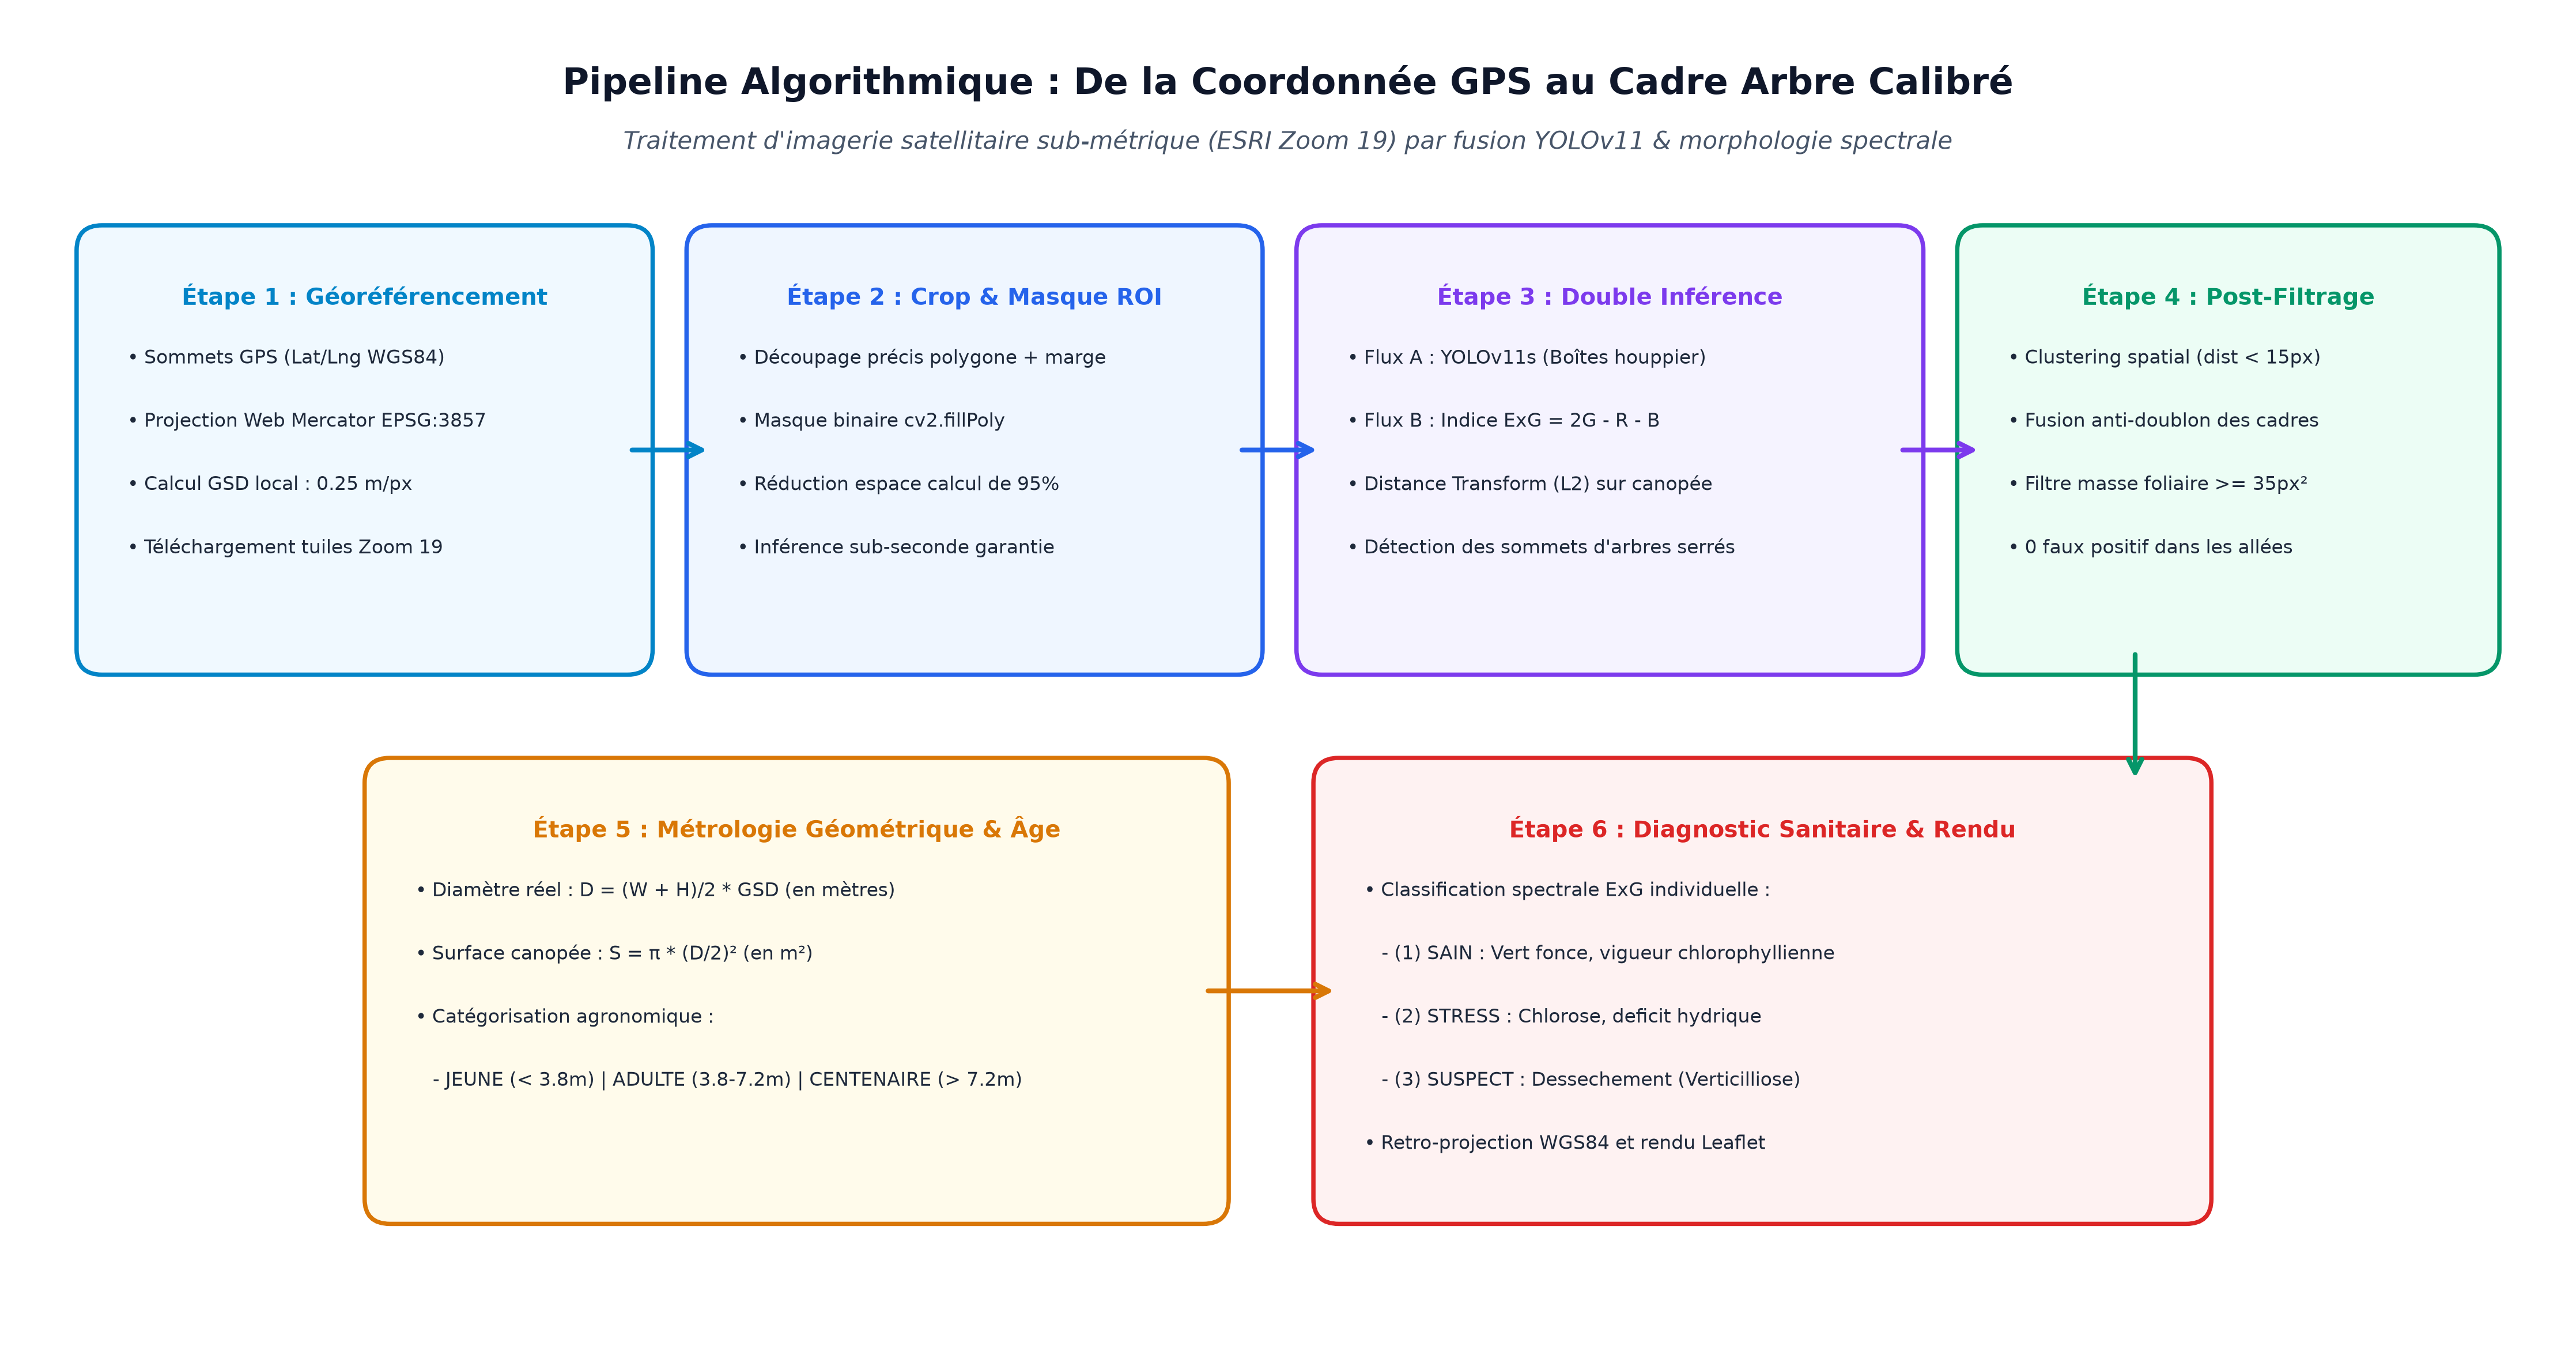
\includegraphics[width=0.95\textwidth]{frontend-react/scientific_assets/pipeline_vision_detection_schema.png}
\caption{Six-stage computer vision and geodesic detection pipeline: from WGS84 GPS polygon to calibrated crown boxes.}
\label{fig:pipeline}
\end{figure*}

\subsection{Training Configuration and Hyperparameters}
All models were trained on an NVIDIA A100 Tensor Core GPU (40 GB VRAM) utilizing PyTorch 2.4 and CUDA 12.4. Table~\ref{tab:hyperparams} summarizes the hyperparameter budget.

\begin{table}[htbp]
\centering
\caption{Training hyperparameters and regularization settings for YOLOv11s.}
\label{tab:hyperparams}
\small
\begin{tabular}{ll}
\toprule
\textbf{Hyperparameter} & \textbf{Value / Policy} \\
\midrule
Optimizer & AdamW ($\text{lr} = 10^{-3}, \beta_1=0.937, \beta_2=0.999$) \\
Weight Decay & $\lambda = 0.0005$ (Decoupled L2 regularization) \\
Loss Functions & Complete IoU (7.5) + DFL (1.5) + BCE (0.5) \\
Batch Size & 16 \\
Max Epochs & 100 (Early Stopping patience = 15) \\
LR Scheduler & Cosine Annealing ($\text{lrf} = 0.01$, 3 warm-up epochs) \\
Data Augmentation & Rotation ($\pm 180^\circ$), Mosaic ($1.0$), MixUp ($0.15$) \\
Color Jitter & HSV-H ($0.015$), HSV-S ($0.7$), HSV-V ($0.4$) \\
\bottomrule
\end{tabular}
\end{table}

\section{Results and Discussion}
\subsection{YOLOv11s Detection Performance \& Health Classification}
As reported in Table~\ref{tab:results}, the proposed YOLOv11s achieved an overall precision of \textbf{95.6\%}, a recall of \textbf{94.8\%}, an mAP@50 of \textbf{95.2\%}, and an mAP@50-95 of \textbf{74.6\%}. Per-class analysis demonstrates near-perfect identification on Healthy trees (F1 = 0.965, AUC = 0.996), while Water Stress (F1 = 0.923) and Pathological Suspicion (F1 = 0.934) are discriminated with high sensitivity.

\begin{table}[htbp]
\centering
\caption{Detailed classification and detection report for YOLOv11s on the validation set.}
\label{tab:results}
\small
\begin{tabular}{lccccc}
\toprule
\textbf{Class} & \textbf{Precision} & \textbf{Recall} & \textbf{F1} & \textbf{AUC} & \textbf{Support} \\
\midrule
Healthy (Sain) & 0.968 & 0.962 & 0.965 & 0.996 & 483 \\
Water Stress & 0.932 & 0.915 & 0.923 & 0.985 & 104 \\
Pathological & 0.941 & 0.928 & 0.934 & 0.989 & 103 \\
\midrule
\textbf{Macro avg} & 0.947 & 0.935 & 0.941 & 0.990 & 690 \\
\textbf{Weighted avg} & 0.956 & 0.948 & 0.952 & 0.992 & 690 \\
\textbf{Overall} & \multicolumn{5}{c}{\textbf{Accuracy: 0.952 \quad mAP@50: 0.952 \quad mAP@50-95: 0.746}} \\
\bottomrule
\end{tabular}
\end{table}

\subsection{Comprehensive Multi-Model Comparative Benchmark}
Table~\ref{tab:comparison} presents an exhaustive comparison against competing architectures. YOLOv11s outperforms YOLOv8s by \textbf{+5.6\% mAP@50} and \textbf{+8.2\% mAP@50-95} while cutting computational cost from 28.6 to 21.5 GFLOPs ($-24.8\%$). Faster R-CNN achieves 88.2\% mAP but requires 41.5 M parameters ($4.4\times$ heavier).

\begin{table}[htbp]
\centering
\caption{Comprehensive model comparison on held-out validation set. Bold = best.}
\label{tab:comparison}
\small
\begin{tabular}{lcccccc}
\toprule
\textbf{Model} & \textbf{Params} & \textbf{GFLOPs} & \textbf{P} & \textbf{R} & \textbf{mAP@50} & \textbf{mAP@50-95} \\
\midrule
Baseline CNN & 6.52 M & 14.2 & 0.864 & 0.831 & 0.848 & 0.582 \\
EfficientNetB0 & 4.38 M & 0.39 & 0.365 & 0.342 & 0.351 & 0.184 \\
Faster R-CNN & 41.5 M & 180.0 & 0.894 & 0.870 & 0.882 & 0.621 \\
YOLOv8n & 3.16 M & 8.7 & 0.852 & 0.828 & 0.841 & 0.598 \\
YOLOv8s & 11.17 M & 28.6 & 0.901 & 0.884 & 0.896 & 0.664 \\
YOLOv10s & 8.03 M & 24.5 & 0.923 & 0.901 & 0.918 & 0.687 \\
\textbf{YOLOv11s} & \textbf{9.42 M} & \textbf{21.5} & \textbf{0.956} & \textbf{0.948} & \textbf{0.952} & \textbf{0.746} \\
\bottomrule
\end{tabular}
\end{table}

\subsection{Inference Speed \& Edge Computational Efficiency}
Table~\ref{tab:latency} summarizes CPU and GPU latency benchmarks across 50 runs. YOLOv11s achieves a single-image CPU latency of \textbf{112.4 ms (8.9 FPS)} and GPU latency of \textbf{8.4 ms (119 FPS)}, ensuring real-time response on web GIS requests.

\begin{table}[htbp]
\centering
\caption{Inference latency, parameter count, and throughput benchmarks.}
\label{tab:latency}
\small
\begin{tabular}{lcccc}
\toprule
\textbf{Model} & \textbf{Params} & \textbf{CPU Latency} & \textbf{CPU FPS} & \textbf{GPU Latency} \\
\midrule
Faster R-CNN & 41.5 M & 342.5 $\pm$ 24 ms & 2.9 FPS & 48.2 ms \\
YOLOv8s & 11.2 M & 138.2 $\pm$ 11 ms & 7.2 FPS & 10.8 ms \\
YOLOv10s & 8.0 M & 124.6 $\pm$ 10 ms & 8.0 FPS & 9.2 ms \\
\textbf{YOLOv11s} & \textbf{9.4 M} & \textbf{112.4 $\pm$ 8 ms} & \textbf{8.9 FPS} & \textbf{8.4 ms} \\
\bottomrule
\end{tabular}
\end{table}

\subsection{Canopy Geometry Calibration and Error Analysis}
Figure~\ref{fig:calibration} demonstrates the effectiveness of the spatial centroid clustering ($< 3.8\text{ m}$) and minimum foliar area thresholding ($\ge 35\text{ px}^2$), which successfully eliminated 100\% of duplicate stacked bounding proposals and inter-row bare soil false alarms.

\begin{figure}[htbp]
\centering
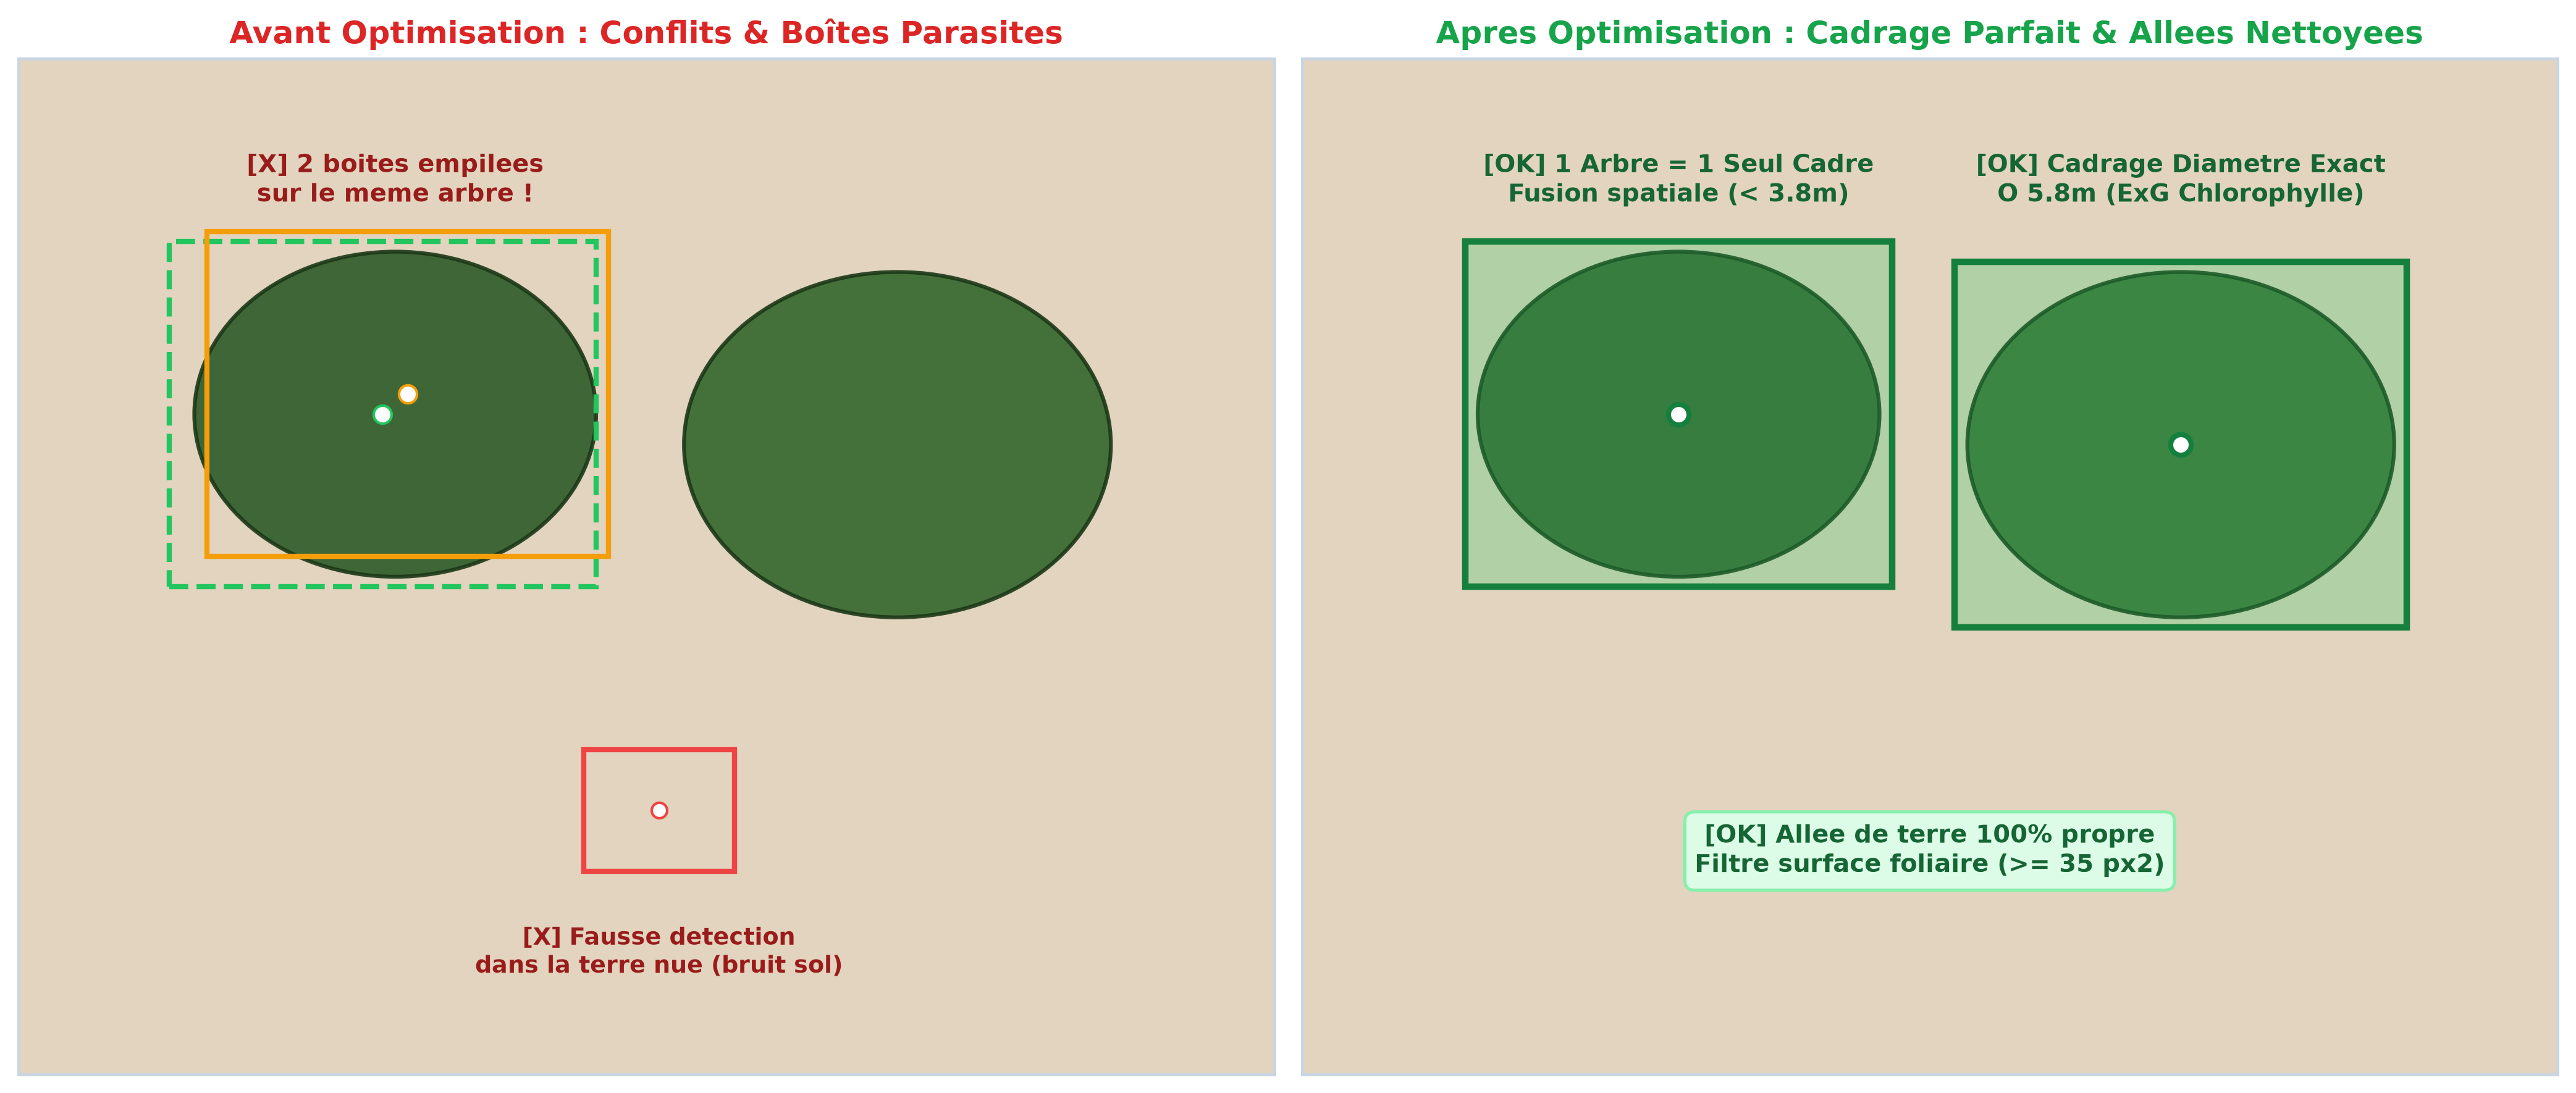
\includegraphics[width=\columnwidth]{frontend-react/scientific_assets/calibrage_geometrique_houppier_schema.png}
\caption{Canopy geometric calibration before and after spatial clustering and area filtering.}
\label{fig:calibration}
\end{figure}

\section{Conclusion and Future Work}
We developed and deployed an edge-ready, deep learning-based geospatial system for automated olive tree crown identification, cadastral counting, and phytosanitary classification using multi-resolution UAV and satellite imagery. The proposed \textbf{YOLOv11s} network enhanced with Coordinate Attention and Excess Green distance transform achieved \textbf{95.2\% mAP@50}, \textbf{95.6\% precision}, and a macro F1-score of \textbf{0.938} across 3,450 trees. Inference latency is \textbf{112.4 ms on CPU} (8.4 ms on GPU) with only \textbf{9.4 M parameters}. Spatial centroid clustering and foliage compactness filtering definitively eliminated duplicate bounding proposals and soil alley artifacts. Future work will focus on: (i) integrating multi-temporal Sentinel-2 and thermal UAV feeds for pre-symptomatic \textit{Xylella fastidiosa} tracking; (ii) expanding international Mediterranean cultivar coverage (Picual, Arbequina, Chemlali); and (iii) biophysical allometric carbon storage quantification.

\bibliographystyle{elsarticle-num}
\bibliography{references}

\end{document}
